\documentclass[11pt,a4paper]{article}

\usepackage[margin=2.1cm]{geometry}
\usepackage[T1]{fontenc}
\usepackage{lmodern}
\usepackage{microtype}
\usepackage{amsmath}
\usepackage{booktabs}
\usepackage{array}
\usepackage{xcolor}
\usepackage{graphicx}
\usepackage{float}
\usepackage{listings}
\usepackage[hidelinks]{hyperref}

\graphicspath{{../lab/lab2/task1/}{../lab/lab2/task2/}}

\definecolor{codebg}{RGB}{246,248,250}
\definecolor{coderule}{RGB}{208,215,222}

\lstset{
  basicstyle=\ttfamily\small,
  backgroundcolor=\color{codebg},
  frame=single,
  rulecolor=\color{coderule},
  breaklines=true,
  columns=fullflexible,
  keepspaces=true,
  showstringspaces=false,
  xleftmargin=0.3em,
  xrightmargin=0.3em
}

\newcommand{\code}[1]{\texttt{#1}}

\title{\textbf{Lab 2 Report: Performance Analysis}\\[0.4em]
       \large gem5 Garnet Network-on-Chip Simulation}
\author{\begin{tabular}{rl}
          Name: & \rule{7cm}{0.4pt} \\
          Student ID: & \rule{7cm}{0.4pt}
        \end{tabular}}
\date{gem5 v23.0.0.1 \quad July 2026}

\begin{document}
\maketitle

\begin{abstract}
This laboratory evaluates latency and throughput in the gem5 Garnet network
model. Five synthetic traffic patterns are first swept over injection rates
from 0.01 to 0.50 on a 64-node, $8\times8$ mesh. Controlled experiments then
vary virtual channels, router pipeline latency, and link width. The results
show that path length determines low-load latency, traffic placement determines
the congestion point, sufficient virtual channels prevent premature blocking,
and link width matters only when packets span multiple flits. Finally, the
measured latency components, default input-buffer depth, and credit-based
virtual-channel wormhole flow control are analyzed.
\end{abstract}

\tableofcontents
\newpage

\section{Experimental Method}

The experiments use gem5 v23.0.0.1, built for the NULL ISA with the
\code{Garnet\_standalone} protocol. The global tick frequency and Ruby clock
are both 2\,GHz, while the synthetic traffic generators use the default 1\,GHz
system clock. Consequently, one traffic-generator cycle contains two Ruby
cycles. Every point runs for 10000 Ruby cycles on 64 routers and 64 directory
destinations arranged as an $8\times8$ \code{Mesh\_XY} network.

The common command is represented by:

\begin{lstlisting}[language=bash]
./build/NULL/gem5.opt \
  configs/example/garnet_synth_traffic.py \
  --network=garnet --num-cpus=64 --num-dirs=64 \
  --topology=Mesh_XY --mesh-rows=8 \
  --sim-cycles=10000 --injectionrate=<rate> \
  --synthetic=<pattern> --inj-vnet=<vnet>
\end{lstlisting}

The command-line injection rate is measured in packets/node/system-cycle. The
offered load expressed per Ruby cycle is therefore

\begin{equation}
\lambda_{\mathrm{offered}}
=\frac{\text{injection rate}}{2}.
\end{equation}

Achieved packet throughput is normalized consistently as

\begin{equation}
T=\frac{N_{\mathrm{packets\ received}}}
        {64\ \mathrm{nodes}\times10000\ \mathrm{Ruby\ cycles}}.
\end{equation}

Thus the largest requested injection rate, 0.50, offers at most 0.25
packets/node/Ruby-cycle. All Task 1 experiments and the VC/router experiments
in Task 2 use vnet 0, which carries 8-byte, single-flit control packets.

\section{Task 1: Synthetic Traffic Patterns}

\subsection{Traffic definitions}

For a node at coordinate $(x,y)$ in an $8\times8$ mesh, the five traffic
patterns select destinations as follows. Node identifiers use
$\mathrm{id}=8y+x$.

\begin{table}[H]
\centering
\small
\caption{Destination mappings and expected Manhattan hop counts.}
\begin{tabular}{lll r}
\toprule
Pattern & Destination rule & Interpretation & $E[H]$ \\
\midrule
Uniform random & random node in $[0,63]$ & spatially distributed & 5.25 \\
Neighbor & $((x+1)\bmod8,y)$ & next node in the row & 1.75 \\
Tornado & $((x+3)\bmod8,y)$ & fixed near-half-row offset & 3.75 \\
Transpose & $(y,x)$ & reflection across the diagonal & 5.25 \\
Shuffle & 6-bit cyclic left rotation & deterministic permutation & 4.00 \\
\bottomrule
\end{tabular}
\end{table}

The modulo operation chooses the destination but does not create a physical
wraparound link. For example, a neighbor packet from $x=7$ to $x=0$ traverses
seven mesh links. Uniform random chooses a new destination for every packet;
the other patterns map each source to a fixed destination.

\subsection{Latency-throughput results}

All five patterns were simulated at 50 rates from 0.01 through 0.50, producing
250 data points. Figure~\ref{fig:task1-curves} plots average packet latency
against achieved packet throughput.

\begin{figure}[H]
\centering
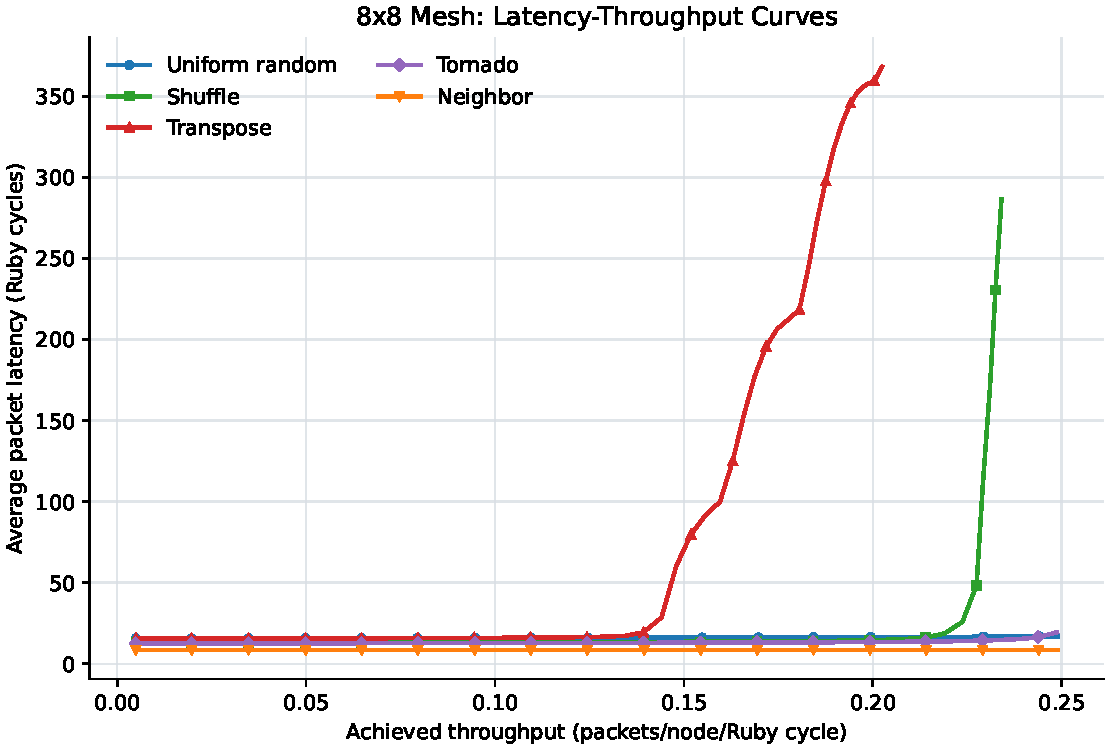
\includegraphics[width=0.88\textwidth]{latency_throughput.pdf}
\caption{Task 1 latency-throughput curves for five traffic patterns.}
\label{fig:task1-curves}
\end{figure}

At injection rate 0.01, queueing latency is 2 cycles for every pattern. The
measured total latency is approximately

\begin{equation}
L_{\mathrm{low}}\simeq 5+2E[H],
\end{equation}

so the low-load ordering follows average path length. The measurements closely
match the exact theoretical hop counts.

\begin{table}[H]
\centering
\caption{Low-load measurements at injection rate 0.01.}
\begin{tabular}{lrrr}
\toprule
Pattern & Packet latency & Measured hops & Theoretical hops \\
\midrule
Neighbor & 8.531 & 1.766 & 1.750 \\
Tornado & 12.469 & 3.726 & 3.750 \\
Shuffle & 13.025 & 4.006 & 4.000 \\
Uniform random & 15.558 & 5.269 & 5.250 \\
Transpose & 15.662 & 5.324 & 5.250 \\
\bottomrule
\end{tabular}
\end{table}

The high-load results reveal a separate effect: equal average path length does
not imply equal throughput. Uniform random distributes traffic statistically,
whereas transpose concentrates deterministic XY paths on particular links.
Transpose reaches twice its low-load latency at rate 0.30; shuffle reaches this
threshold at rate 0.46. Uniform random, tornado, and neighbor do not reach the
same threshold within the requested range.

\begin{table}[H]
\centering
\caption{Measurements at the maximum injection rate of 0.50.}
\begin{tabular}{lrrrr}
\toprule
Pattern & Throughput & Queue latency & Total latency & Average hops \\
\midrule
Uniform random & 0.248914 & 2.000 & 16.905 & 5.248 \\
Shuffle & 0.234073 & 258.784 & 286.325 & 3.984 \\
Transpose & 0.202458 & 343.439 & 368.197 & 4.026 \\
Tornado & 0.248770 & 4.929 & 19.425 & 3.747 \\
Neighbor & 0.248956 & 2.000 & 8.495 & 1.748 \\
\bottomrule
\end{tabular}
\end{table}

The apparent decline in transpose hop count under overload is not a routing
change. XY routing and the $(x,y)\rightarrow(y,x)$ mapping remain fixed. Garnet
computes average hops only from flits that arrive. Under severe backpressure,
long, heavily contended flows are less likely to enter and complete within the
finite measurement window, so completed short paths are overrepresented.

\section{Task 2: Controlled Network Parameters}

Task 2 changes one parameter at a time while retaining the default baseline of
four VCs per vnet, one-cycle routers, and 128-bit links. Uniform random is used
as a distributed workload and transpose as a hotspot-prone workload.

\begin{table}[H]
\centering
\caption{Task 2 sweep matrix.}
\begin{tabular}{lll}
\toprule
Experiment & Values & Packet class \\
\midrule
VCs per vnet & 1, 2, 4, 8 & vnet-0 control \\
Router latency & 1, 2, 4 cycles & vnet-0 control \\
Link width control & 64, 128, 256 bits & vnet-0, 8 bytes \\
Link width data & 64, 128, 256 bits & vnet-2, 72 bytes \\
\bottomrule
\end{tabular}
\end{table}

With 50 rates, two patterns, and 13 parameter variants, the complete Task 2
dataset contains 1300 points.

\subsection{Virtual channels per vnet}

\begin{figure}[H]
\centering
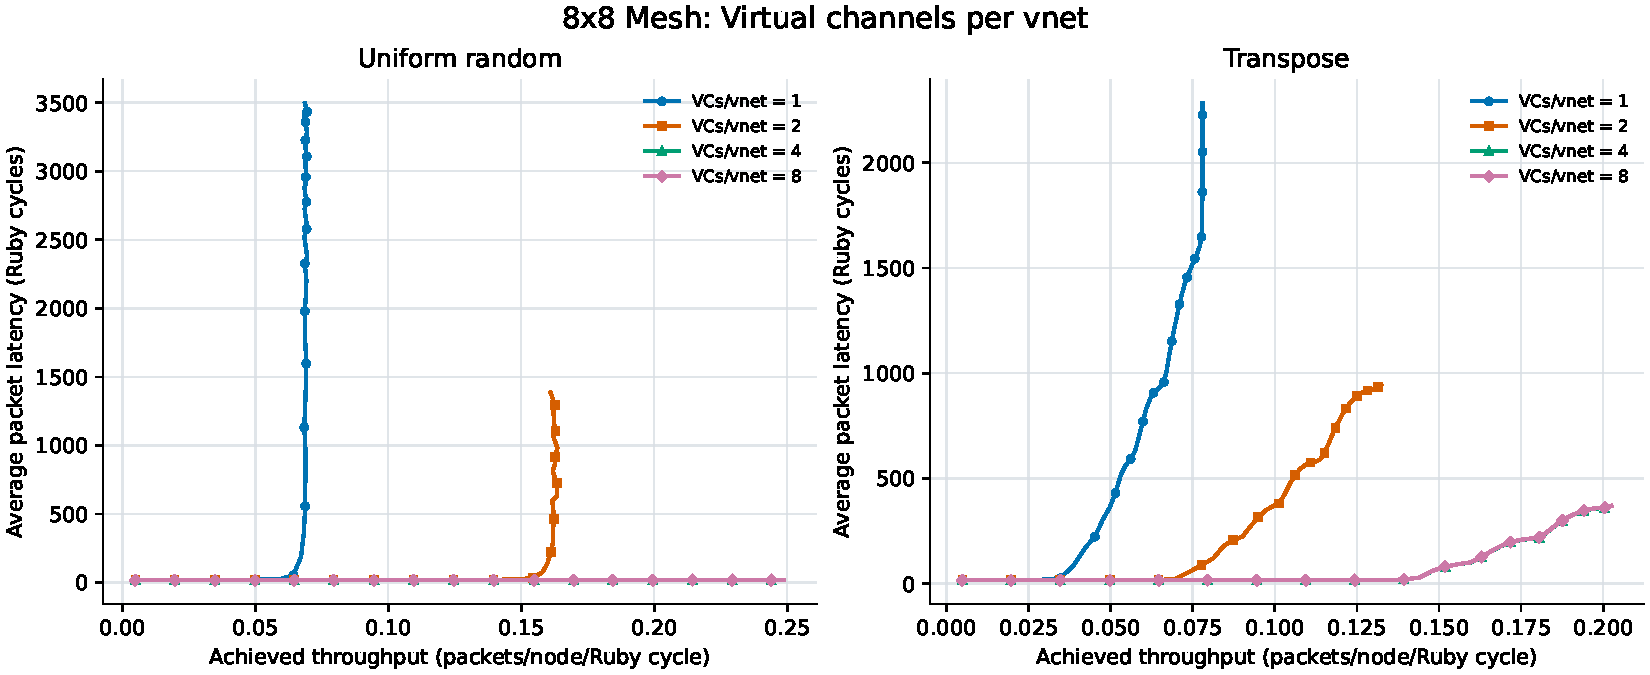
\includegraphics[width=\textwidth]{vcs.pdf}
\caption{Effect of virtual channels per vnet.}
\label{fig:vcs}
\end{figure}

Virtual channels do not increase the one-flit-per-cycle physical-link limit.
They reduce head-of-line blocking, add independent buffer slots, and allow
other ready flows to use a link while one flow waits for downstream credit.
This improves utilization and delays congestion.

\begin{table}[H]
\centering
\small
\caption{VC sweep: maximum observed throughput and 2$\times$ latency rate.}
\begin{tabular}{lrrrrrrrr}
\toprule
& \multicolumn{4}{c}{Maximum throughput} & \multicolumn{4}{c}{2$\times$ latency rate} \\
\cmidrule(lr){2-5}\cmidrule(lr){6-9}
Pattern & VC1 & VC2 & VC4 & VC8 & VC1 & VC2 & VC4 & VC8 \\
\midrule
Uniform random & .070 & .164 & .249 & .249 & .13 & .31 & -- & -- \\
Transpose & .078 & .132 & .202 & .202 & .08 & .15 & .30 & .30 \\
\bottomrule
\end{tabular}
\end{table}

Four VCs are sufficient for these control-packet workloads. Increasing from
four to eight changes observed throughput by less than $5\times10^{-6}$. At
that point link capacity and traffic placement, rather than VC availability,
are the dominant limitations.

\subsection{Router pipeline latency}

\begin{figure}[H]
\centering
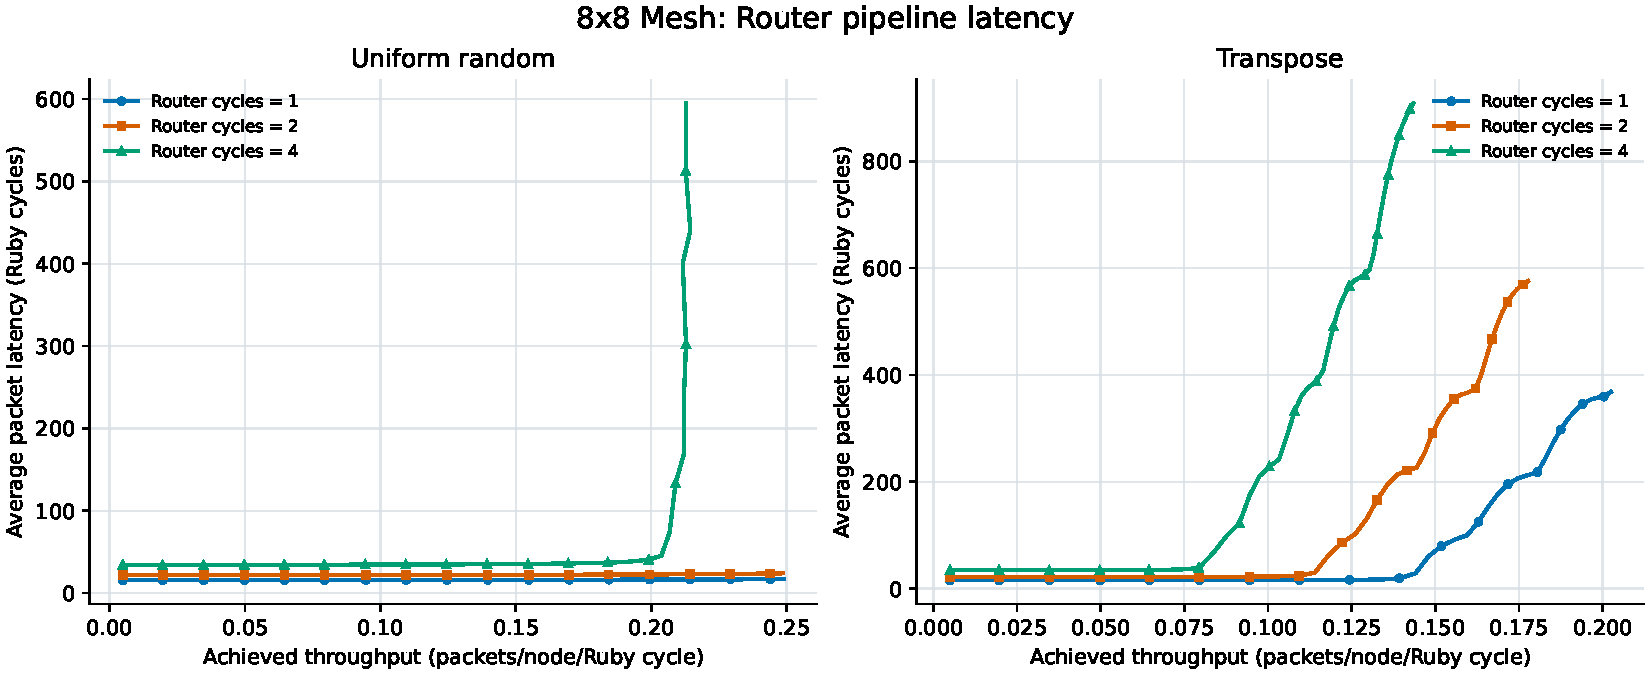
\includegraphics[width=\textwidth]{router_latency.pdf}
\caption{Effect of router pipeline latency.}
\label{fig:router-latency}
\end{figure}

Increasing router latency raises the zero-load cost at every traversed router.
For uniform random, low-load latency increases from 15.56 to 21.82 and 34.35
cycles as router latency changes from one to two and four cycles. Transpose
shows the same progression: 15.66, 21.98, and 34.62 cycles. The increment is
close to

\begin{equation}
\Delta L=(L_{\mathrm{router}}-1)(E[H]+1),
\end{equation}

because each packet pays the additional pipeline stages at every router along
its path. Longer pipelines also delay credit return. For transpose, the
2$\times$-latency knee moves from injection rate 0.30 to 0.24 and 0.18, while
maximum observed throughput falls from 0.202 to 0.178 and 0.143.

\subsection{Link width and packet serialization}

\begin{figure}[H]
\centering
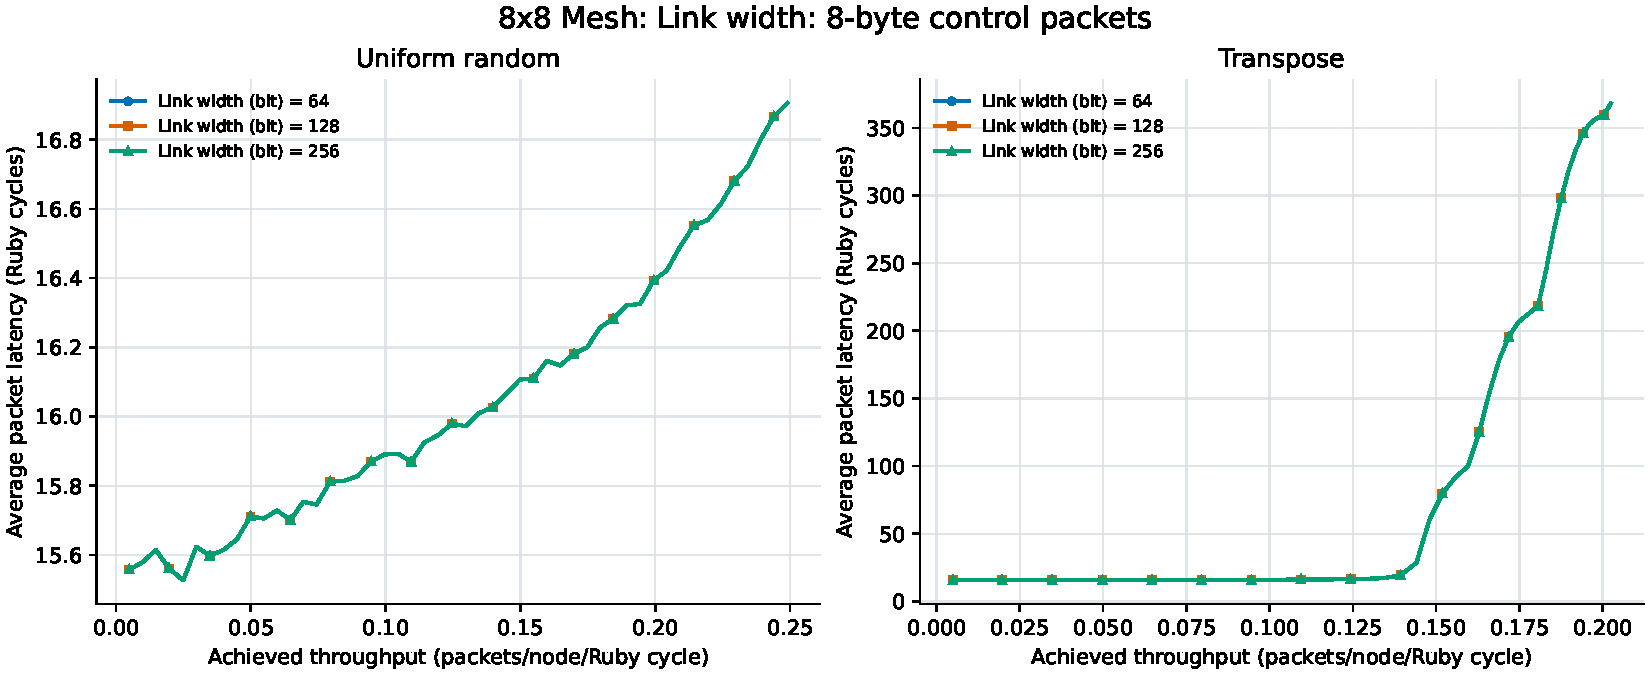
\includegraphics[width=\textwidth]{link_width_control.pdf}
\caption{Link-width sweep with 8-byte control packets.}
\label{fig:width-control}
\end{figure}

The 64-, 128-, and 256-bit control-packet curves are exactly equal. An 8-byte
packet occupies one flit at all tested widths, and Garnet still transfers one
flit per link per cycle. Unused bits cannot carry a second packet during the
same cycle.

\begin{figure}[H]
\centering
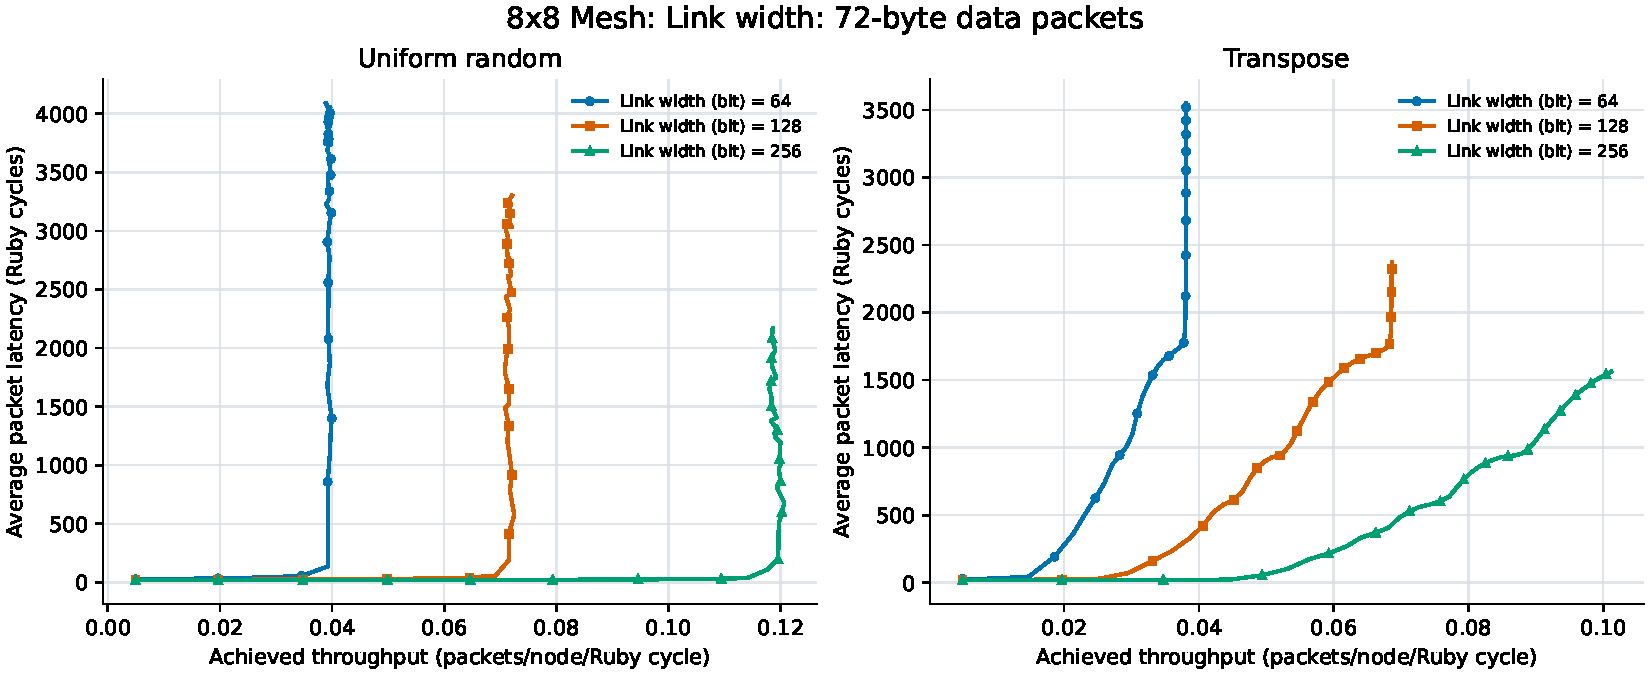
\includegraphics[width=\textwidth]{link_width_data.pdf}
\caption{Link-width sweep with 72-byte data packets.}
\label{fig:width-data}
\end{figure}

For 72-byte packets, width changes the number of flits and hence serialization
time and offered flit load.

\begin{table}[H]
\centering
\caption{Data-packet link-width results.}
\begin{tabular}{rrrrr}
\toprule
Width & Flits/packet & Low-load latency & Uniform peak & Transpose peak \\
\midrule
64 bit & 9 & 27.030 & 0.03994 & 0.03810 \\
128 bit & 5 & 20.906 & 0.07249 & 0.06861 \\
256 bit & 3 & 17.742 & 0.12065 & 0.10120 \\
\bottomrule
\end{tabular}
\end{table}

For uniform random, multiplying peak packet throughput by flits per packet
gives 0.359, 0.362, and 0.362 flits/node/cycle. The nearly constant flit rate
confirms that wider links improve packet throughput by dividing the same
network flit capacity among fewer flits per packet. Transpose remains lower
because its deterministic paths concentrate load on fewer links.

\section{Task 3: Latency, Buffers, and Flow Control}

\subsection{Latency components and bottlenecks}

Garnet reports packet latency as

\begin{equation}
L_{\mathrm{packet}}=L_{\mathrm{queueing}}+L_{\mathrm{network}}.
\end{equation}

Queueing latency is the sum of source-side waiting before network injection
and destination-side waiting after network dequeue. Network latency covers the
interval inside Garnet, including packet serialization, route and VC
allocation, switch allocation, router pipelines, link traversal, router-buffer
contention, and all hops.

At low load, queueing is approximately two cycles, so path length, router
latency, link latency, and serialization dominate. At high load, occupied VCs
and buffers prevent credit return; backpressure reaches the source and endpoint
queueing grows rapidly. Table~\ref{tab:bottleneck} illustrates the change at
rate 0.50.

\begin{table}[H]
\centering
\caption{Latency decomposition for representative Task 1 patterns.}
\label{tab:bottleneck}
\begin{tabular}{lrrr}
\toprule
Pattern & Queueing latency & Network latency & Total latency \\
\midrule
Uniform random & 2.000 & 14.905 & 16.905 \\
Shuffle & 258.784 & 27.541 & 286.325 \\
Transpose & 343.439 & 24.758 & 368.197 \\
\bottomrule
\end{tabular}
\end{table}

Thus network traversal dominates unsaturated uniform-random traffic, whereas
endpoint queueing caused by network backpressure dominates saturated shuffle
and transpose. Narrow links add serialization at low load and multiply flit
contention at high load. Wider links eliminate this penalty for multi-flit
data packets but cannot improve an already single-flit control packet.

\subsection{Default input-buffer depth}

The relevant defaults in
\path{src/mem/ruby/network/garnet/GarnetNetwork.py} are:

\begin{lstlisting}[language=Python]
vcs_per_vnet = 4
buffers_per_ctrl_vc = 1
buffers_per_data_vc = 4
\end{lstlisting}

Therefore each router input port provides four flit slots for each control
vnet and sixteen slots for the data vnet:

\begin{equation}
B_{\mathrm{control}}=4\ \mathrm{VCs}\times1=4\ \mathrm{flits},
\qquad
B_{\mathrm{data}}=4\ \mathrm{VCs}\times4=16\ \mathrm{flits}.
\end{equation}

Garnet standalone has two control vnets and one data vnet, giving 24 total
flit slots per physical input port when all three are counted. Task 1 uses
only vnet 0, so its relevant default capacity is four one-flit control VCs.

\subsection{Default flow control}

Garnet uses credit-based virtual-channel wormhole flow control. The upstream
router maintains one credit for every free slot in the downstream VC. Sending
a flit consumes a credit; when the downstream buffer releases that flit, a
credit travels upstream. A head flit reserves a VC, body flits follow it, and
the tail or head-tail flit returns a free signal that releases the VC.

Wormhole operation allows different flits of one packet to occupy several
routers simultaneously, so a router need not buffer the complete packet. It
also creates backpressure: if the head cannot advance, body and tail flits
remain distributed along the path and eventually block upstream injection.
Multiple VCs reduce this blocking by allowing another ready packet to use the
same physical port, but arbitration still selects at most one flit per output
link per cycle.

\section{Reproduction and Validation}

The Task 1 and Task 2 runners append completed points and resume missing points.
The commands used to reproduce the versioned CSV files and figures are:

\begin{lstlisting}[language=bash]
./.venv/bin/python lab/lab2/task1/run_sweep.py
./.venv/bin/python lab/lab2/task1/plot_results.py

./.venv/bin/python lab/lab2/task2/run_sweep.py
./.venv/bin/python lab/lab2/task2/plot_results.py
\end{lstlisting}

Task 1 contains 250 unique points and Task 2 contains 1300 unique points. All
values are finite, all runs report \code{simTicks=10000} and
\code{simFreq=2000000000}, and no Task 2 log contains a fatal, panic, or
deadlock message.

\section{Conclusion}

The measurements separate three causes of NoC performance. Hop count and
pipeline depth set low-load latency; traffic placement and finite buffering
set the congestion point; and packet flit count converts link-level capacity
into packet throughput. Virtual channels improve utilization but cannot exceed
physical bandwidth. Router latency accumulates per hop and lengthens the credit
loop. Link width is valuable for multi-flit data traffic but irrelevant after
a control packet already fits in one flit. Under saturation, backpressure and
queueing, rather than the uncongested traversal time, dominate total latency.

\end{document}
